\providecommand{\main}{../../../..}
\documentclass[\main/dresen_thesis.tex]{subfiles}

\begin{document}
  \label{sec:monolayers:preparation:nanoparticleVariation}
    \begin{figure}[tb]
      \centering
      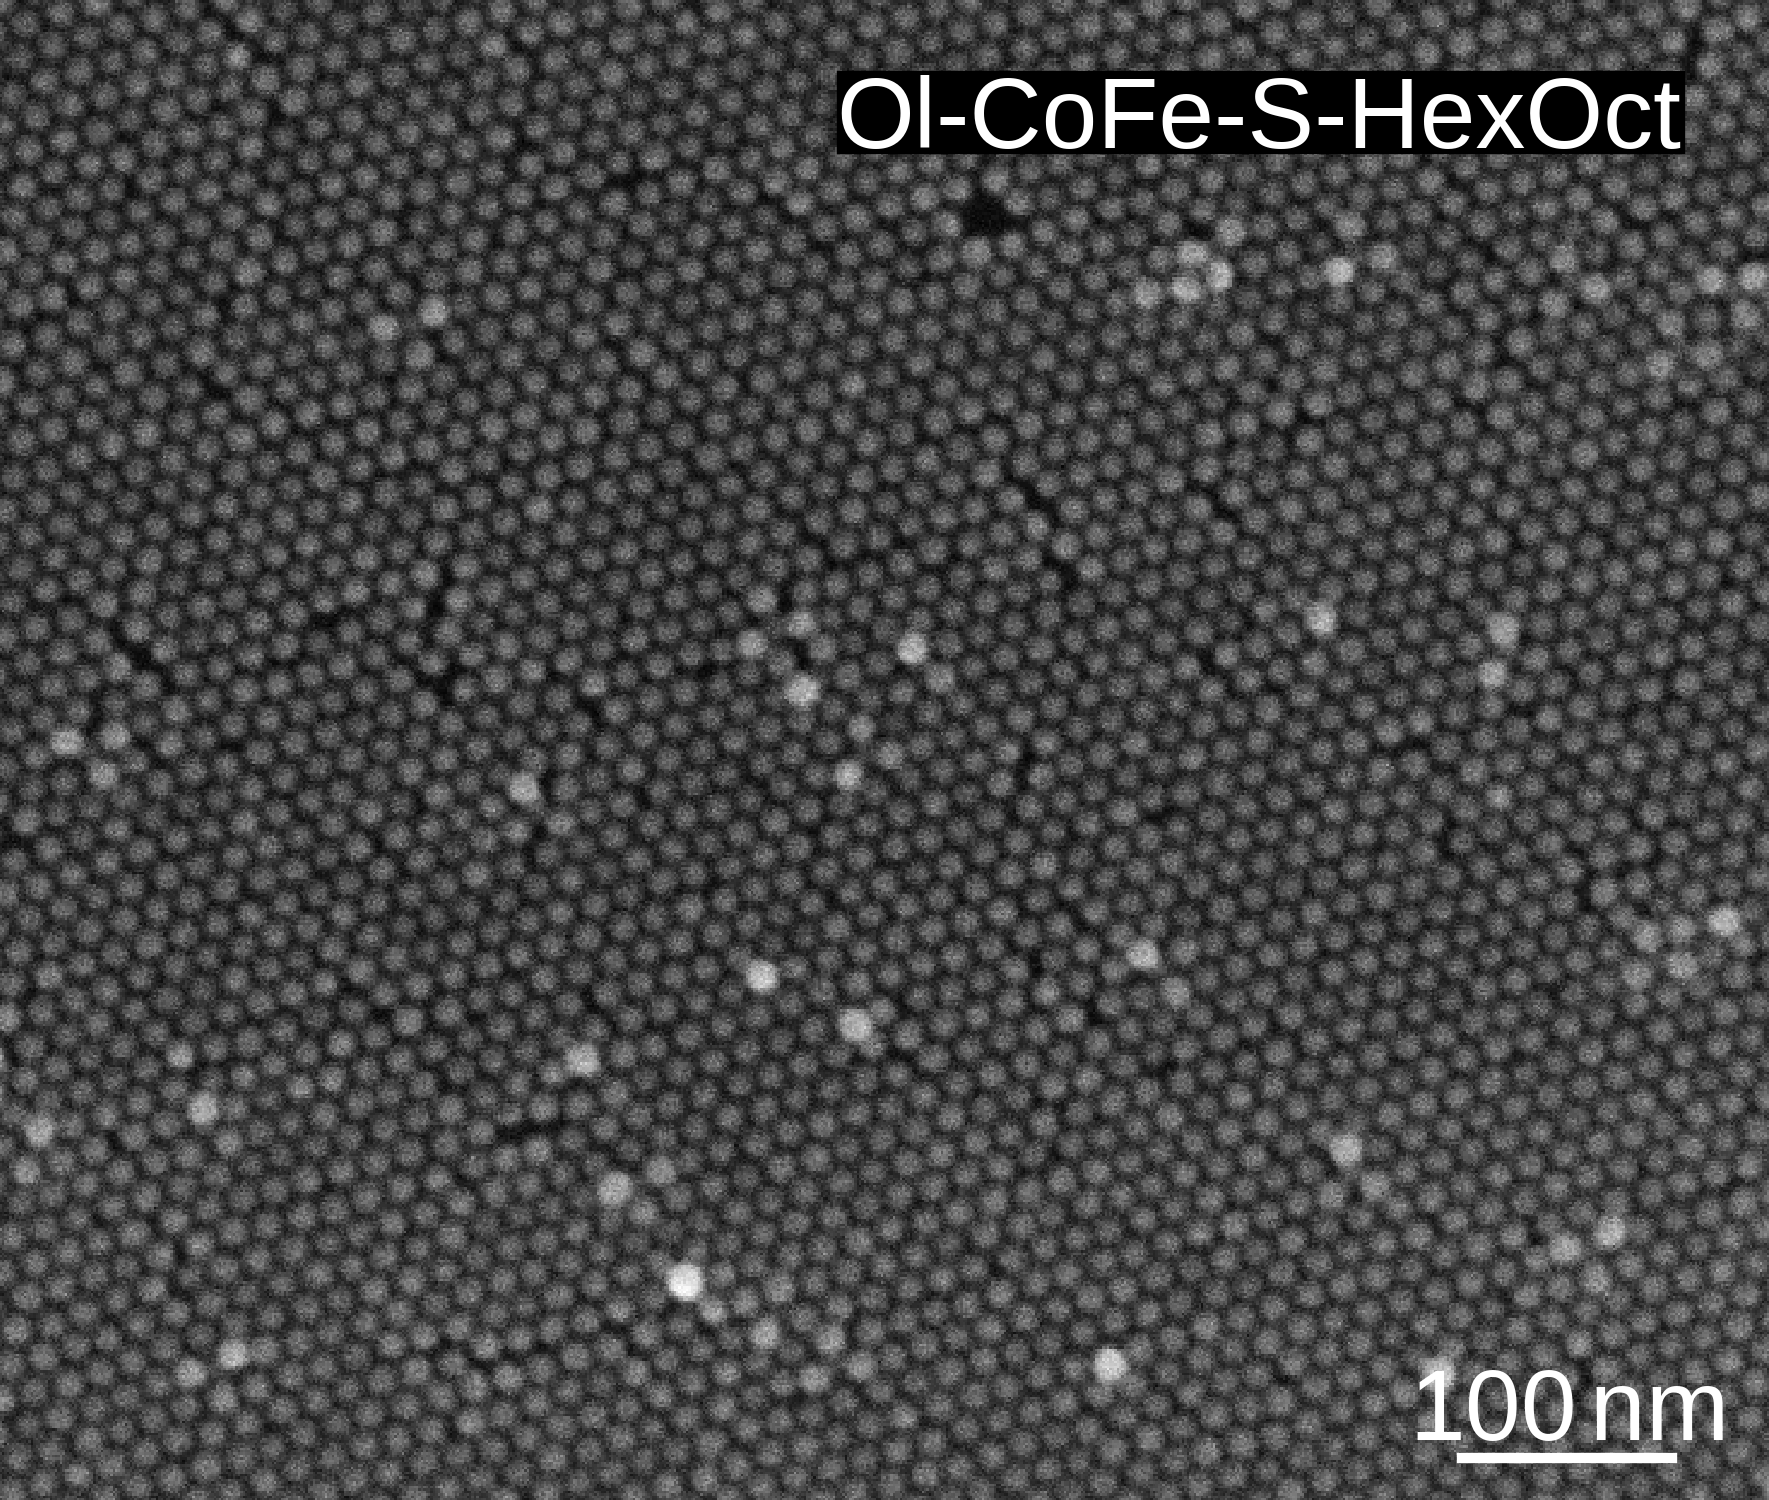
\includegraphics{monolayers_SEM_Ol-CoFe-S-HexOct}
      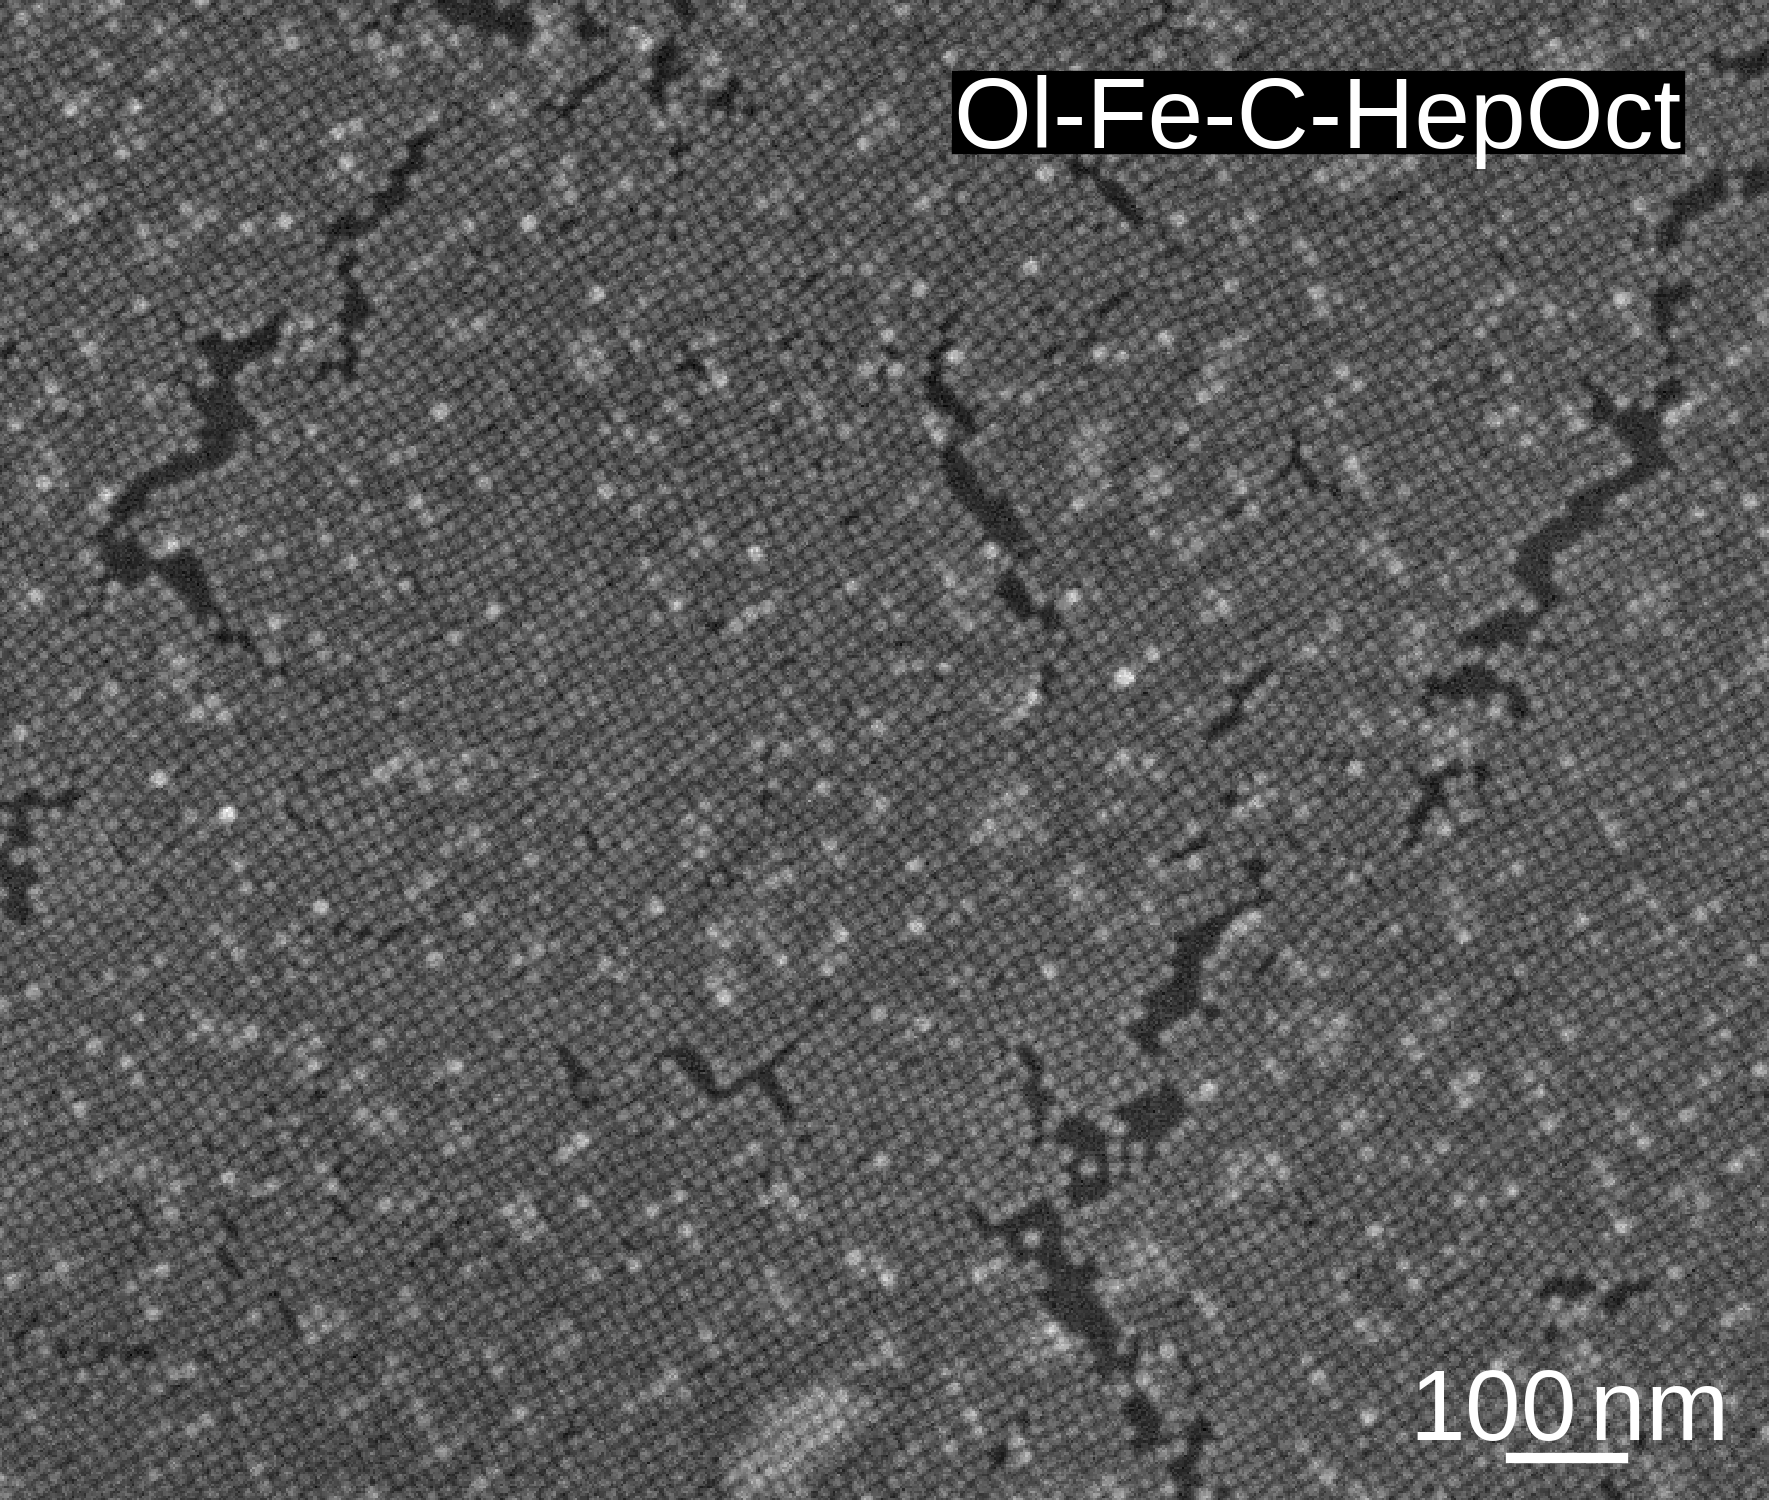
\includegraphics{monolayers_SEM_Ol-Fe-C-HepOct}
      \caption{\label{fig:monolayers:preparation:nanoparticleVariation:spheresIron}Scanning electron microscopy of other type of nanoparticles deposited as monolayers also using 1-octadecene as co-solvent. Shown is the structure of cobalt ferrite nanospheres (left) and iron oxide nanocubes (right).}
    \end{figure}
\end{document}